% Especificaciones del tamaño de letra, tamaño de hoja, márgenes, librerias, etc.
\documentclass[12pt, letterpaper]{article}
\usepackage[english]{babel}
\usepackage[utf8]{inputenc}
\usepackage[T1]{fontenc}
\usepackage{amsmath}
\usepackage{graphicx}
\usepackage{subcaption}
\usepackage{hyperref}
\usepackage{url}
\usepackage{amssymb}
\usepackage{float}
\usepackage[margin=1in]{geometry}
\renewcommand{\baselinestretch}{1.5}

% Enlace Bibliografía
\usepackage{csquotes}
\usepackage[notes,backend=biber]{biblatex-chicago}
\addbibresource{referencias.bib}

% Titulo, autores, fecha.
\title{Práctica \#6: Análisis de Deformación}
\author{Carlos Vásquez 1155057}

% Inicio del documento
\begin{document}
\maketitle
\section*{Introducción}

El análisis de deformaciones que sufre un material es muy importante ya que, dado que las dimensiones cambian dependiendo del esfuerzo que éste sufra, puede que herramientas compuestas que se deformen más allá de lo tolerable y la máquina/objeto se vuelva inutilizable. Por eso es de gran utilidad realizar estos cálculos y obtener una deformación aproximada para así diseñar nuestros sistemas y herramientas con estas consideraciones.

\section*{Desarrollo}

Analizar estas deformaciones es sencillo, lo que haremos será realizar un análisis de nuestro objeto compuesto en SOLIDWORKS. Nuestro objeto está conformado por la siguiente figura:

\begin{figure}[H]
	\centering
	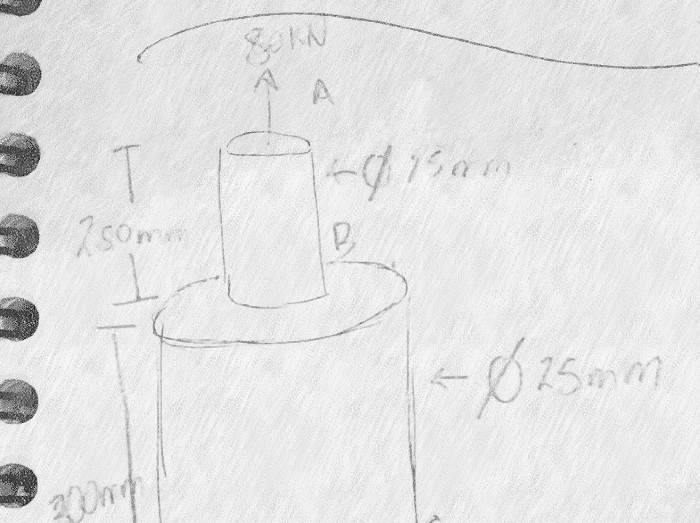
\includegraphics[width=0.7\textwidth]{ph.jpg}
	\caption{Diagrama de los cilindros.}
\end{figure}

Esta figura está hecha del metal \textit{AISI 1045 estirado en frío}, el cual tiene un módulo de elasticidad de 205 GPa. Si modelamos todo el objeto en SOLIDWORKS y aplicamos la carga mostrada en la figura (de 80 kN), obtendremos los siguientes datos:

\begin{figure}[H]
	\centering
	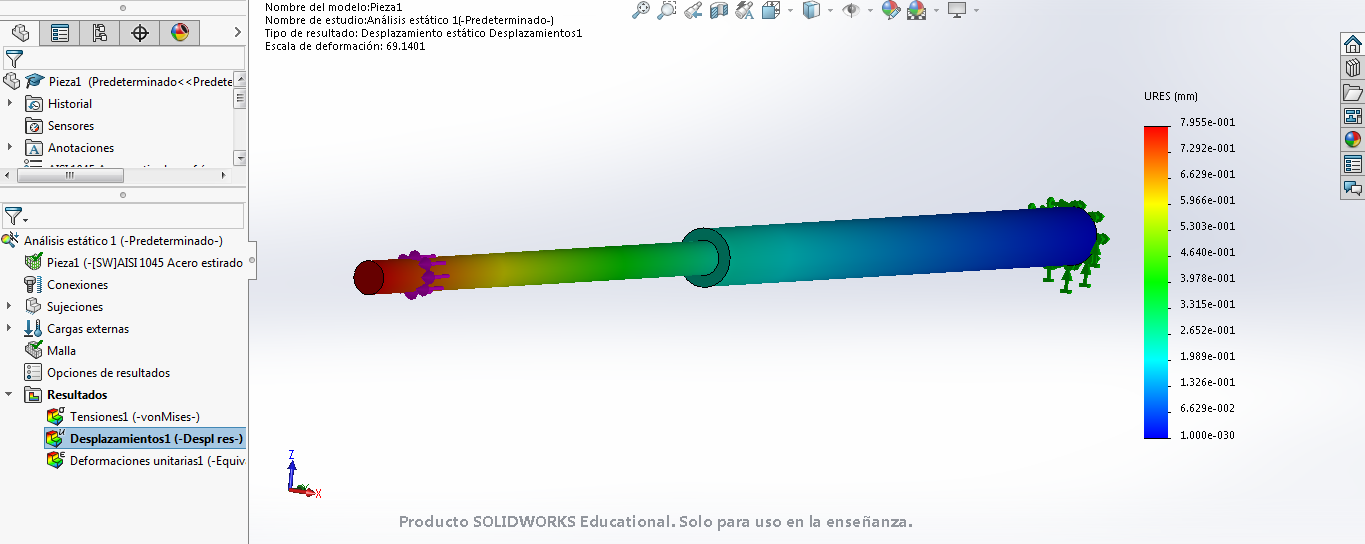
\includegraphics[width=\textwidth]{deft.PNG}
	\caption{Deformación total del objeto.}
\end{figure}

\begin{figure}[H]
	\centering
	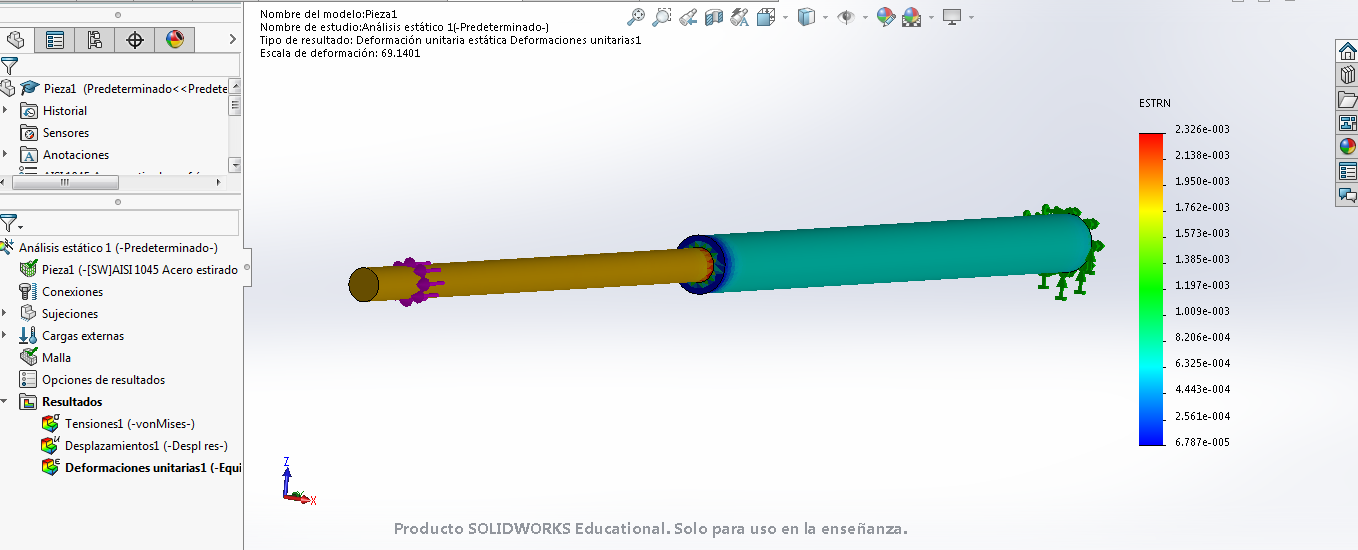
\includegraphics[width=\textwidth]{defu.PNG}
	\caption{Deformación unitaria de las barras.}
\end{figure}

\begin{figure}[H]
	\centering
	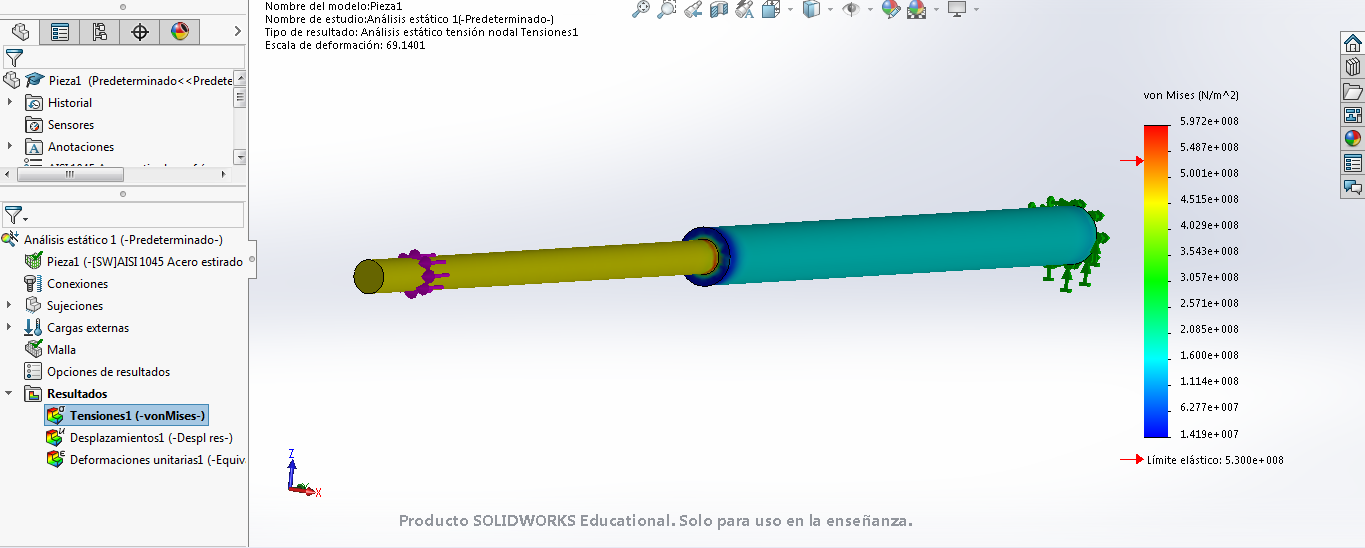
\includegraphics[width=\textwidth]{von.PNG}
	\caption{Análisis de von Mises para la barra completa.}
\end{figure}

\section*{Cálculos} 

Ahora bien, si deseamos realizar los cálculos de deformación lo único que debemos de conocer es que $\sigma \propto \epsilon$. La constante de proporcionalidad es el módulo de elasticidad del material, usualmente determinado de manera experimental. Entonces nuestra ecuación, conocida como ley de Hooke, quedará expresada de la siguiente manera:
\begin{equation}
	\sigma = E \epsilon
\end{equation}

Sin embargo, recordamos que la fórmula para la deformación unitaria es:

\begin{equation}
	\epsilon = \frac{\delta}{L}
\end{equation}

Dadas estas dos relaciones anteriores, podemos obtener que:

\begin{equation}
	\delta = \frac{PL}{EA}
\end{equation}

Hecho este análisis, podemos proceder a realizar el análisis de la barra compuesta. Dado queel material es el mismo para la barra de diámetro mayor y menor, entonces el módulo de elasticidad es el mismo para ambas. Lo que debemos de tomar en consideración es que, como tienen un diámetro distinto, será preciso analizar la deformación total de cada barra y después obtener la total mediante la suma aritmética de ambas, de la siguiente manera:

\begin{equation}
	\delta_T = \delta_{AB} + \delta_{BC}
\end{equation}

Para obtener cada una de las deformaciónes realizaremos sólo sustituimos los valores que ya conocemos en la ecuación 3.

\begin{equation}
	\begin{split}
		\delta_{BC} &= \frac{(80,000\ N)(0.3\ m)}{(205,000,000,000\ Pa)(1.5625\pi \times 10^{-4}\ m^2)}\\
		\delta_{BC} &= 2.3849 \times 10^{-4}\ m
	\end{split}
\end{equation}

\begin{equation}
	\begin{split}
		\delta_{AB} &= \frac{(80,000\ N)(0.25\ m)}{(205,000,000,000\ Pa)(5.625\pi \times 10^{-5}\ m^2)}\\
		\delta_{AB} &= 5.5208 \times 10^{-4}\ m
	\end{split}
\end{equation}

Por lo tanto, nuestra deformación total será la suma de los resultados de la ecuación 5 y 6.
\begin{equation}
	\boxed{\delta_T = 7.9057 \times 10^{-4} m}
\end{equation}

\section*{Conclusión}
Si observamos la deformación total del objeto en la simulación, veremos que el valor de ésta es bastante cercano al valor calculado con la fórmula idealizada de deformación a partir de la ley de Hooke. Sin embargo, como en otras prácticas ha sido mencionado, debemos de recordar que nuestro análisis ha sido ideal. Al momento de considerar la geometría de una manera más real, así coo considerar otros factores, entonces nuestra deformación puede cambiar bastante. A pesar de esto, SOLIDWORKS realiza una muy buena estimación y es realmente efectivo para cálculos rápidos, en especial cuando la geometría se vuelve mucho más compleja.

%%%%%  Bib
\renewcommand\refname{Referencias}
\printbibliography
\end{document}
